\section{Durchführung}
\label{sec:Durchführung}


\subsection{Untersuchung der Funktionsweise eines Lock-In-Verstärkers}
Um die generelle Funktionsweise des Lock-In-Verstärkers zu untersuchen wird die Schaltung aus \autoref{fig:lock_in_amplifier_2} aufgebaut.
Wobei im ersten Teil des Versuches der Noisegenerator ausgeschaltet ist damit die Abhängigkeit zwischen der Phase und der Ausgangsspannung untersucht werden kann.
Dazu werden die Ausgangsspannungen für 10 verschiedene Phasen gemessen.
Im zweiten teil des ersten Versuches werden die 10 Messungen mit eingeschaltetem Noisegenerator wiederholt um den Einfluss
des Rauschens auf die Spannung zu untersuchen.

\begin{figure}
  \centering
  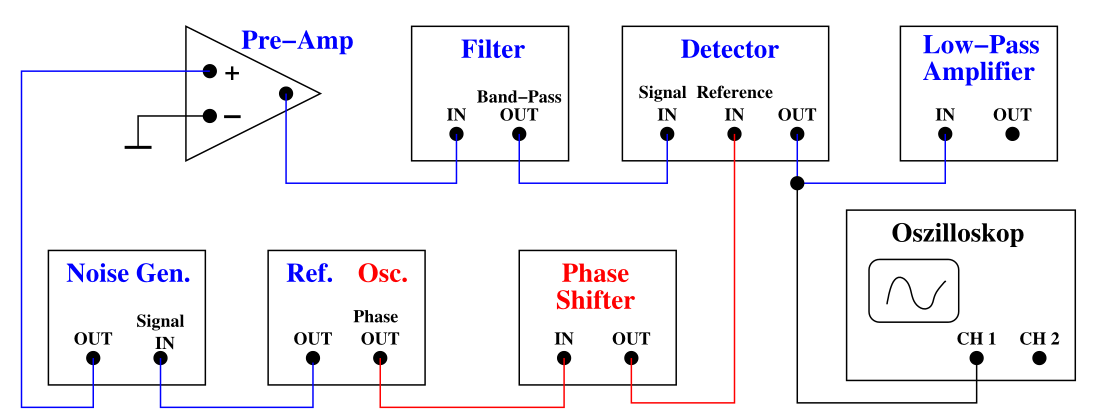
\includegraphics[scale=0.4]{assets/lock_in_amplifier_2.png}
  \caption{Schematischer Aufbau des Lock-In-Verstärkers \cite{V303}}
  \label{fig:lock_in_amplifier_2}
\end{figure}


\subsection{Photodetektorschaltung}
Um die Lichtintensität einer LED trotz Umgebungslichtes messen zu können wird jetzt die Schaltung aus \autoref{fig:lock_in_amplifier_3} aufgebaut.


\begin{figure}
  \centering
  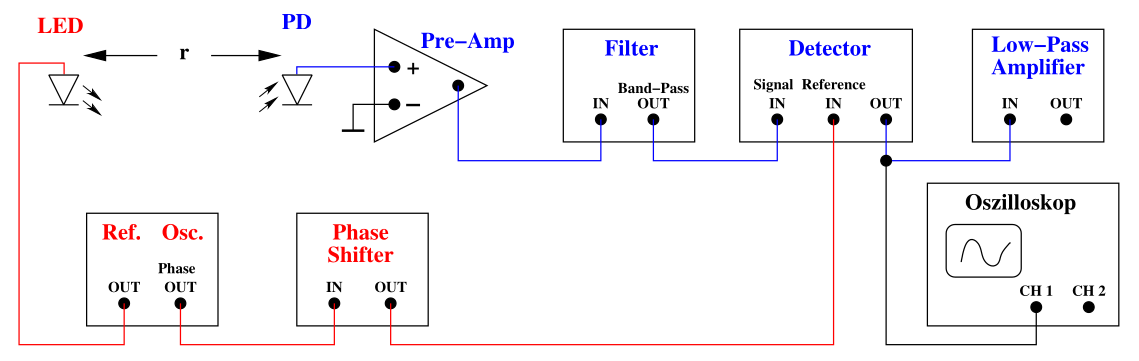
\includegraphics[scale=0.4]{assets/lock_in_amplifier_3.png}
  \caption{Schematischer Aufbau der Photodetektorschaltung zur Untersuchung der Lichtintensität der LED. \cite{V303}}
  \label{fig:lock_in_amplifier_3}
\end{figure}

\noindent Mit dieser wird jetzt für immer größer werdende Abständen, zwischen LED und Detektor, die Spannungen am Ausgang des Tiefpassfilters gemessen.

% \begin{figure}
%   \centering
%   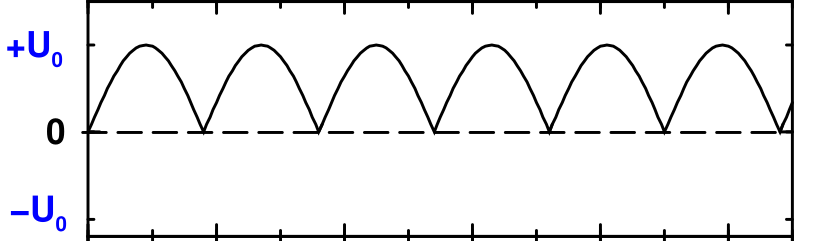
\includegraphics[scale=0.5]{assets/example_1.png}
%   \caption{Ausgangssignal\cite{V303}}
%   \label{fig:example_1}
% \end{figure} 